%%%%%%%%%%%%%%%%%%%% author.tex %%%%%%%%%%%%%%%%%%%%%%%%%%%%%%%%%%%
%
% sample root file for your "contribution" to a contributed volume
%
% Use this file as a template for your own input.
%
%%%%%%%%%%%%%%%% Springer %%%%%%%%%%%%%%%%%%%%%%%%%%%%%%%%%%


% RECOMMENDED %%%%%%%%%%%%%%%%%%%%%%%%%%%%%%%%%%%%%%%%%%%%%%%%%%%
\documentclass[graybox]{svmult}

% choose options for [] as required from the list
% in the Reference Guide

\usepackage{mathptmx}       % selects Times Roman as basic font
\usepackage{helvet}         % selects Helvetica as sans-serif font
\usepackage{courier}        % selects Courier as typewriter font
\usepackage{type1cm}        % activate if the above 3 fonts are
                            % not available on your system
%
\usepackage{makeidx}         % allows index generation
\usepackage{graphicx}        % standard LaTeX graphics tool
                             % when including figure files
\usepackage{multicol}        % used for the two-column index
\usepackage[bottom]{footmisc}% places footnotes at page bottom

\usepackage{newunicodechar}
\usepackage{program}

% see the list of further useful packages
% in the Reference Guide

\makeindex             % used for the subject index
                       % please use the style svind.ist with
                       % your makeindex program

%%%%%%%%%%%%%%%%%%%%%%%%%%%%%%%%%%%%%%%%%%%%%%%%%%%%%%%%%%%%%%%%%%%%%%%%%%%%%%%%%%%%%%%%%

\begin{document}

\title*{eMDPM: EFFICIENT MULTI-DIMENSIONAL
PATTERN MATCHING ALGORITHM FOR GPU}
\titlerunning{eMDPM}
% Use \titlerunning{Short Title} for an abbreviated version of
% your contribution title if the original one is too long
\author{Supragya Raj$^{\alpha}$, Siddha Prabhu Chodnekar$^{\alpha}$ , Harish T$^{\alpha}$ and Harini Sriraman$^{\alpha}$}
\authorrunning{Supragya Raj, S.P Chodnekar, Harish T, Harini S.}
% Use \authorrunning{Short Title} for an abbreviated version of
% your contribution title if the original one is too long
\institute{Supragya Raj \at SCSE, VIT Chennai$^{\alpha}$, \email{supragyaraj@gmail.com}
\and Siddha Prabhu Chodnekar$^{\alpha}$, Harish T$^{\alpha}$, Harini Sriraman$^{\alpha}$, \newline\email{sprabhu.chodnekar@vit.ac.in}, \email{harini.s@vit.ac.in}
\newline\newline
${\alpha}$: School of Computing Science and Engineering, Vellore Institure of Technology, Chennai Campus, Chennai
600127, India}
%
% Use the package "url.sty" to avoid
% problems with special characters
% used in your e-mail or web address
%
\maketitle

\abstract*{Each chapter should be preceded by an abstract (10--15 lines long) that summarizes the content. The abstract will appear \textit{online} at \url{www.SpringerLink.com} and be available with unrestricted access. This allows unregistered users to read the abstract as a teaser for the complete chapter. As a general rule the abstracts will not appear in the printed version of your book unless it is the style of your particular book or that of the series to which your book belongs.
Please use the 'starred' version of the new Springer \texttt{abstract} command for typesetting the text of the online abstracts (cf. source file of this chapter template \texttt{abstract}) and include them with the source files of your manuscript. Use the plain \texttt{abstract} command if the abstract is also to appear in the printed version of the book.}

\abstract{Parallelizing pattern matching in multi-dimensional images is very vital in many applications to improve performance. With SIMT architectures, the performance can be greatly enhanced if the hardware threads are utilized to the maximum. In case of pattern matching algorithms, the main bottle neck arises due to the reduction operation that needs to be performed on the multiple parallel search operations. This can be solved by using Shift-Or operations. Recent trend has shown the improvement in pattern matching using Shift-Or operations for bit pattern matching. This has to be extended for multiple dimensional images like hyper-cubes. In this paper, we have extended the shift-or pattern matching for multi-dimensional images. The algorithm is implemented for GPU architectures. The complexity of the proposed algorithm is $ m*\frac{log(n)}{kw} $ where $m$ is the number of dimensions, $n$ is the size of the array if the multidimensional matrix values are placed in a single dimensional array, $k$ is the size
of the pattern and w is the size of the tile. From the result analysis it is found that the performance is maximum, when the pattern size matches the tile size and it is less than 64. This restriction is due to the size of the warp considered.\newline\newline\textbf{Keywords} Pattern Matching, Parallelism, GPU, Shift-Or operations}

\section{Introduction}
\label{sec:1}
With advent of GPUs, execution time of image processing applications has greatly reduced. Pattern searching is an integral part of many applications. Any improvement in the performance of pattern matching of multi-dimensional image will greatly improve the performance of many GPU based applications. Pattern matching can be broadly classified into exact bit pattern matching and approximate bit pattern matching algorithms. The main bottle neck with respect to improving the performance pattern searching is reduction operation. In recent times, shift–or operation is used to improve the efficiency of reduction operation based pattern matching algorithms.

Parallel pattern matching involves tasks identification, communication identification, task agglomeration and mapping of tasks to processors. GPU is a SIMT architecture that can be utilized effectively for pattern matching algorithms. The matching of individual patterns can happen in the stream processors available inside the stream multiprocessors. The communication involves the reduction process. Agglomeration and mapping depends on the number of processors available. If we consider $n$ to be the number of primitive tasks and $p$ to be the number of processors, then $\frac{n}{p}$ tasks can be assigned per processor.
\section{Related Work}
\label{sec:2}
% Always give a unique label
% and use \ref{<label>} for cross-references
% and \cite{<label>} for bibliographic references
% use \sectionmark{}
% to alter or adjust the section heading in the running head
Pattern matching involves the process of identifying all patterns in a given text. There are many practical applications in which pattern matching algorithms are applied. The pattern matching algorithms can be classified with respect to the dimensions of the data. Further classification of these algorithms include the type of pattern matching namely, exact pattern
matching and approximate pattern matching.

\subsection{Exact and approximate pattern matching}
\label{subsec:2}
Exact pattern matching provides a solution by viewing each text position to be a possible pattern start. For exact pattern matching algorithm, the complexity is O(mn) where m*n is the dimension of the text matrix. Many improvements exist in the literature for exact pattern matching algorithms. Usage of linear automata [1] for the purpose is the most popular technique. This reduces the complexity of the pattern matching algorithm to be O(m+n). Good-suffix heuristic algorithm proposed in [2] provides an improved performance of O(n) with constant space requirement. In [3], bad character rule strategy is generalized and improves the performance of the pattern matching algorithm with time complexity of O(n/m). Simple pattern searching algorithm proposed in [4] improves the average time complexity to be O(m+n).

Approximate parallel pattern matching algorithms works on the principle that a error can be tolerated by the pattern match. Say for example if a particular pattern match algorithm with pattern size of ‘m’ can tolerate ‘n’ error bits, approximate pattern matching algorithm will find out all the matches with ‘m to m-n’ matching bits. This matching will be particularly useful for bigger images. Parallelizing of the above categories of algorithms can be performed in different ways. This is highlighted in section 2.2.

\subsection{Parallel bit pattern matching algorithms}
\label{subsec:2}

Approximate and exact pattern matching algorithms falls into the category of finite and non-deterministic automata. Parallelizing these algorithms for better performance has evolved and there are many perspectives to this in the literature. Parallel algorithms that consider bit pattern mapping for parallelization is described in this section.

Many traditional algorithms like Shift-Or[9] and Shift-And[10] algorithms form the basis of almost all Deterministic Finite State automata based pattern matching algorithms. These finite state automata are stored in form of bits. Hence, for pattern text of size $n$, there are $n$ bits to store all the prefixes of match in the text.  Algorithms such as KMP are a good example of this. Recent work in the domain of pattern matching like Bit Parallel Wide window[12] and Backward Non Deterministic Matching [11] reduces the $n$ bits requirements in favour of computation cost. These research directions are based on the idea that matches in strings of large alphabet size is often sparse and not all prefixes are needed to be stored for the matching.

Reverse factor[5], linear DAWG matching[6], BSDM using Q-Grams and shift-xor[7] and Two way shift-or[13] are manifestations of the popular Shift-Or algorithm itself and apply the domain specific constraints to efficiently parallelise the shift-or algorithm.

\section{eMDPM Algorithm}
\label{sec:3}
% Always give a unique label
% and use \ref{<label>} for cross-references
% and \cite{<label>} for bibliographic references
% use \sectionmark{}
% to alter or adjust the section heading in the running head

The eMDMP algorithm rests heavily on the developments done in[1] and takes over much of these concepts to build upon in this paper. The nomenclature and a few of the terms that are used in the algorithm that follows are:

\begin{itemize}
\item{$M$ are used for denoting masks. Masks are state storing variables and can take any of 2\textsuperscript{n} combination of bits. They are 0 wherever there is a match of certain character and 1 otherwise. This mask is then reversed. For instance in string "AABAB", the mask M\textsubscript{A} is 10100 (swapped from 00101, the positions of A).}
\item{R is the residue vector, bit of which denote the matching of all prefixes of pattern P on text T. (See p3 [1] for further reading). }
\item{$\langle a,b \rangle$ denotes the binary operator [dot] used in SO exact matching. (see p5 [1] for further reading). }
\item{$a \vert b$ denotes the Shift-Or operations done in cuShiftOr. This takes advantage of multiple threads and computing S matrix. The S matrix denote the residual values extracted from R. X is the final result vector. }
\end{itemize}

\subsection{Proposed algorithm}
\label{subsec:1}

\textbf{Input}: A text $T$ of n\textsubscript{1} x n\textsubscript{2} and pattern $P$ of m\textsubscript{1} x m\textsubscript{2} \newline
\textbf{Output}: A matrix $X$ of size (n\textsubscript{1} - m\textsubscript{1} + 1) x (n\textsubscript{2} - m\textsubscript{2} + 1) indicating matching positions

\begin{program}
\BEGIN \\ %
	Initialise .. Masks .\textsl{M}\textsubscript{1}\textsl{, M}\textsubscript{2}\textsl{, ... M}\textsubscript{n}. for .the .test .image .T.
  \FOR i:=\textsl{1} \TO \textsl{n\textsubscript{1}-m\textsubscript{1}-1} \DO
  	\FOR j:=\textsl{0} \TO \textsl{m\textsubscript{1}-1} \DO
  	A\textsubscript{0}:= \langle \textsl{0,1}\textsuperscript{\textsl{m}} \rangle
  	A\textsubscript{k}:= \langle \textsl{1,M}\textsubscript{\textsl{k}} \rangle for.all.k.in.\textsl{0 $\leq$ k $\leq$ n1}
  		\FOR k:=\textsl{0} \TO \textsl{n\textsubscript{2}} \DO in parallel
  			R\textsubscript{k}:= sum(\textsl{A}\textsubscript{0}\textsl{,A}\textsubscript{1}\textsl{,...A}\textsubscript{k}) \rcomment{Inclusive Scan}
  		\END
  		\langle \textsl{u}\textsubscript{\textsl{k}} \textsl{,S}\textsubscript{\textsl{j,k}}\rangle:= R\textsubscript{k} ..for.all..\textsl{0 $\leq$ k $\leq$ n2}
  	\END
  	\FOR j:=\textsl{m2} \TO \textsl{n2} \DO
  		y\textsubscript{j}:= \textsl{S}\textsubscript{i,j}\vert\textsl{S}\textsubscript{i+1,j}\vert\textsl{...}\vert\textsl{S}\textsubscript{i+m1-1,j} \rcomment{Shift-Or}
  		X[i][j\textsl{-}m\textsubscript{2}\textsl{+1}]:= y\textsubscript{j}[m\textsubscript{2}]
 	\END
 \END
\END
\end{program}


An example run of the above given algorithm can be summarised using the following figure ~\ref{fig:1}.
\begin{figure}
\sidecaption
% Use the relevant command for your figure-insertion program
% to insert the figure file.
% For example, with the graphicx style use
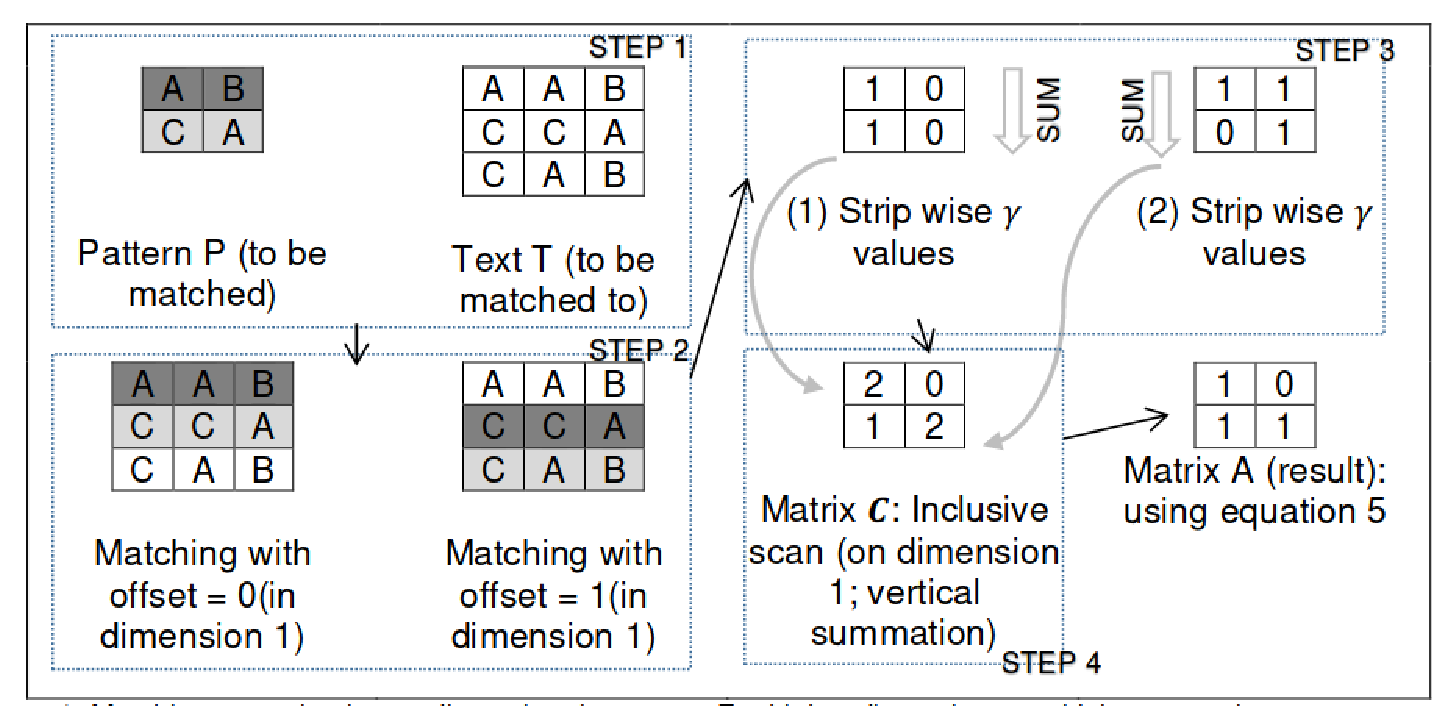
\includegraphics[scale=.50]{workingsys.eps}
%
% If no graphics program available, insert a blank space i.e. use
%\picplace{5cm}{2cm} % Give the correct figure height and width in cm
%
\caption{Matching operation in two dimensional systems. For higher dimensions, multiple summations occur to gather matrix C; first on dimension 1 to give intermediate set C1; on them, summation on dimension 2 is done etc. Process continues till all dimensions are summed upon to give final C, hence A}
\label{fig:1}       % Give a unique label
\end{figure}


\subsection{Tile based data decomposition}
\label{subsec:3}
Tile based data decomposition is used for improved performance in the GPU. Tiles of size $w*w$ are shared among multiple SPs(Stream Processors) for processing .This improves the performance by reducing the redundant reads otherwise needed in the system. The parallelism is performed by considering the data are stored as a single linear array of values. The single linear array values are then loaded to the shared memory of the SP to be used by multiple threads of the same block. To synchronize the operation, after each tile read, a $\_\_syncthreads()$ function is called for performing a barrier like wait till all the threads in the same block has completed loading input to the tile. In the considered algorithm, this tile based data load has greatly improved the performance of the system. The data update is done in the shared memory is shown in the following figure.

\begin{figure}
\sidecaption
% Use the relevant command for your figure-insertion program
% to insert the figure file.
% For example, with the graphicx style use
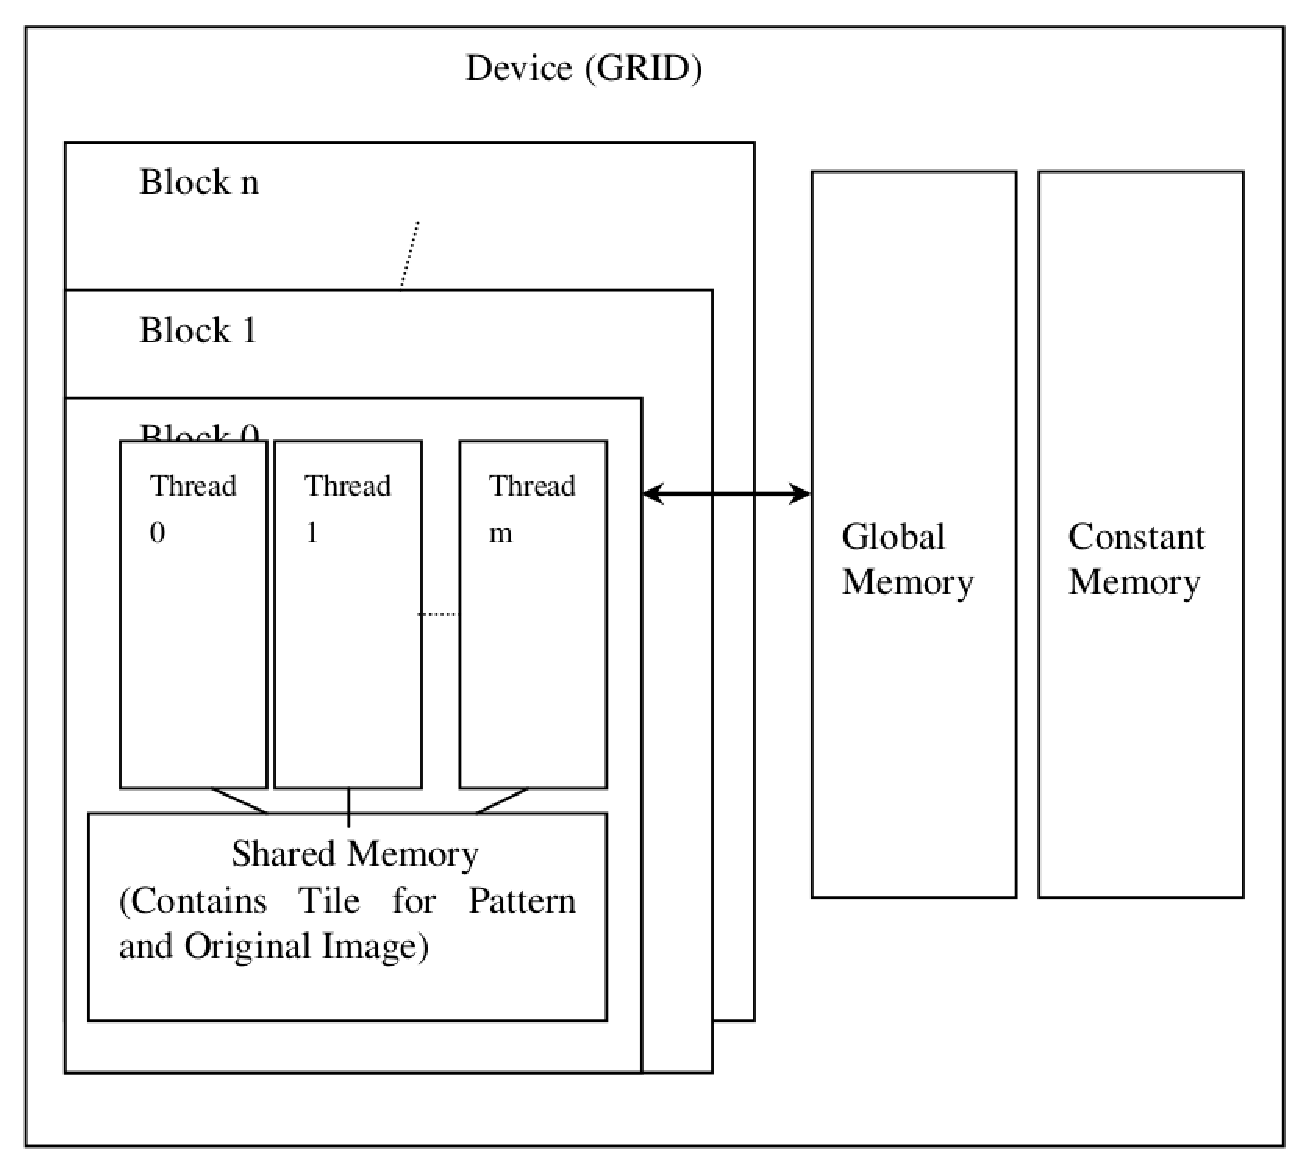
\includegraphics[scale=.50]{GPUin.eps}
%
% If no graphics program available, insert a blank space i.e. use
%\picplace{5cm}{2cm} % Give the correct figure height and width in cm
%
\caption{Storing of image and pattern as tile in shared memory of GPU}
\label{fig:2}       % Give a unique label
\end{figure}

\section{Result and analysis}
\label{sec:4}
For multi-dimensional images, pattern matching algorithms has plenty of possibility to parallelize. This helps in utilizing the GPU to the maximum and improves the performance of the algorithm. The main overhead with respect to parallelism is the increased communication overhead. But in the proposed implementation, the latency of this access is reduced by utilizing the shared memory. For the implemented system, the CGMA (Compute to Global Memory Access) ratio is 3:1. The compute for global
memory access includes the following list of tasks.

\begin{itemize}
\item{Shift-Or operation to perform pattern matching}
\item{Or operation to update row-wise results of the tile}
\item{Reduction with multiple rows}
\end{itemize}

In the above case, row wise operations are performed with in thread of the tile. This can also be performed with respect to columns.

Let $m$ be the number of dimensions of the image considered, $n$ represents the total image size, $k$ represents the size of the pattern and $w$ represents the dimension of the tile. The time complexity of the proposed algorithm is given by:

$$
Execution time = \left( m \times \frac{log_w(k)}{wlog(n)} \right)
$$

Comparison between the performances of proposed algorithm with cuShiftOr is shown in Fig. 10. The performance of the proposed algorithm is better when the pattern size is less than 64 and the tile size matches the pattern size.

\begin{figure}
\sidecaption
% Use the relevant command for your figure-insertion program
% to insert the figure file.
% For example, with the graphicx style use
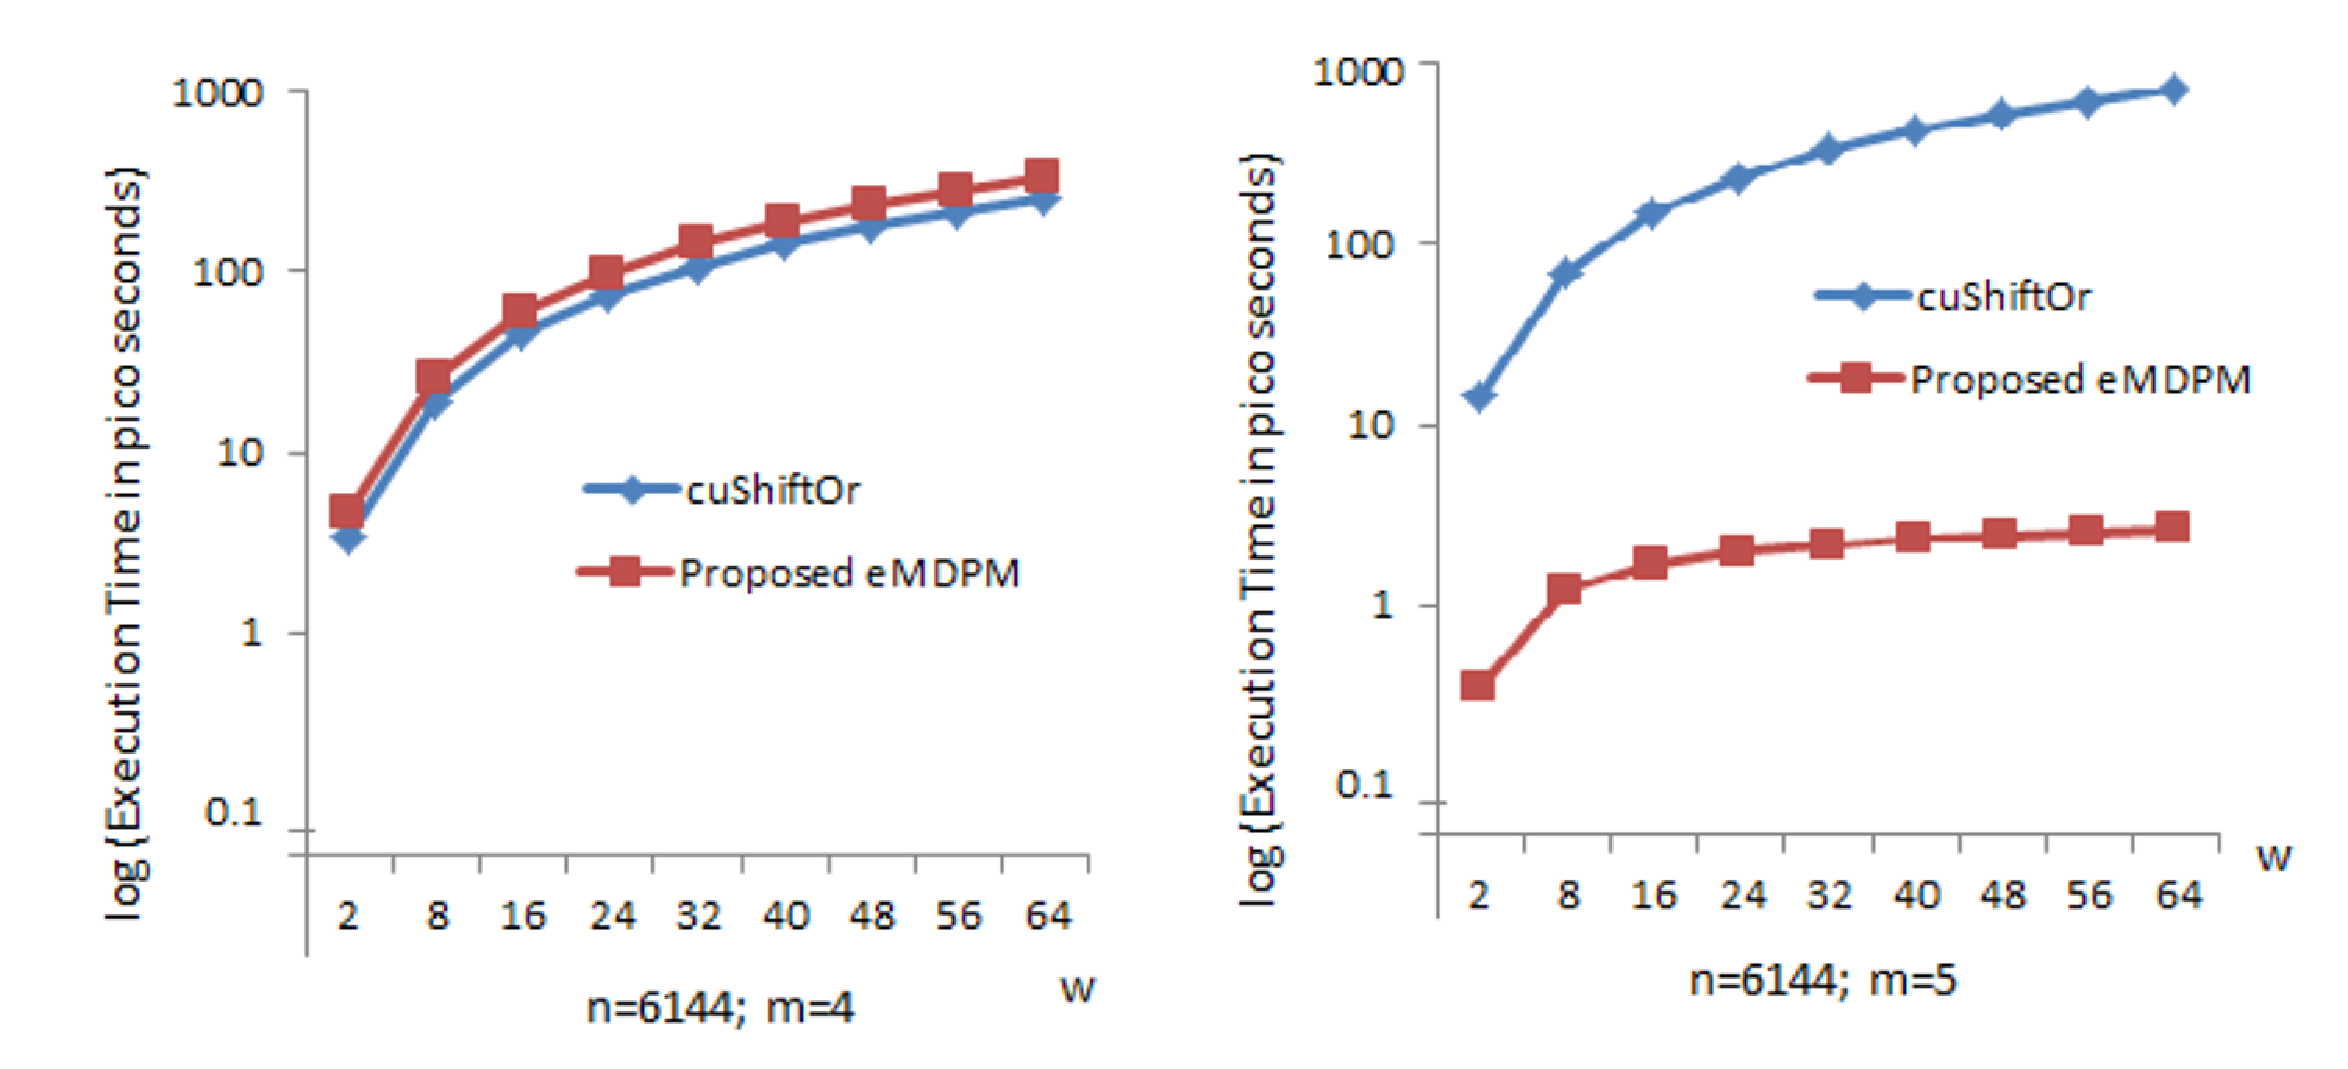
\includegraphics[scale=.29]{compare0.eps}
%
% If no graphics program available, insert a blank space i.e. use
%\picplace{5cm}{2cm} % Give the correct figure height and width in cm
%
\caption{Comparison between cuShiftOr and eMDPM on dimensions 4 and 5.}
\label{fig:2}       % Give a unique label
\end{figure}

In the Fig 3, the performance of eMDPM algorithm for different values of $w$ is shown. For this analysis, $n$ is considered to be 6144 and $m$ is set to be 3. For other values also, the algorithm can be analysed. Here for a sample $m$ and $n$ the analysis is shown.

\begin{figure}
\sidecaption
% Use the relevant command for your figure-insertion program
% to insert the figure file.
% For example, with the graphicx style use
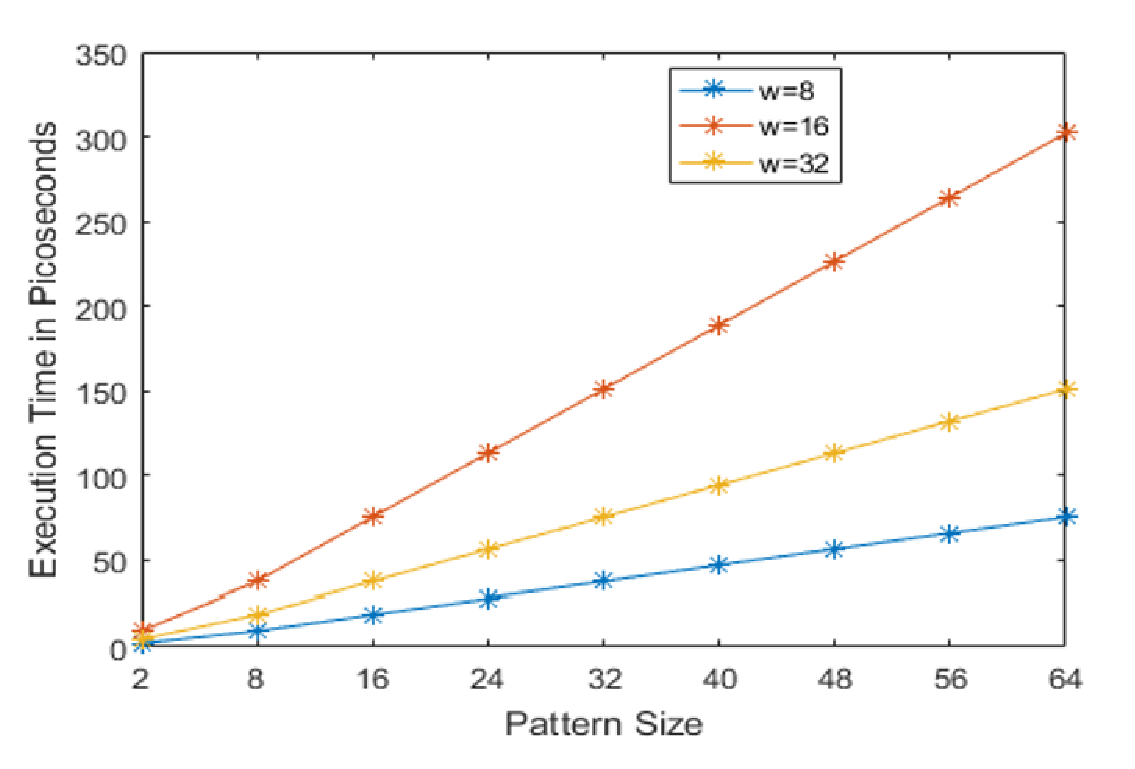
\includegraphics[scale=.49]{executiontime.eps}
%
% If no graphics program available, insert a blank space i.e. use
%\picplace{5cm}{2cm} % Give the correct figure height and width in cm
%
\caption{eMDPM : Execution Time Versus Tile Size}
\label{fig:3}       % Give a unique label
\end{figure}

\section{Conclusion and future work}
\label{sec:5}
In this paper an efficient multi-dimensional parallel pattern matching algorithm is proposed and analyzed. The performance of the proposed algorithm with multidimensional images is much improved compared to existing algorithms. The implementation of the proposed algorithm is done using GPU. The proposed algorithm works well with GPU architecture by increasing CGMA ratio. Proposed algorithm makes use of tiles for data caching which improves the performance of pattern matching in GPU based architectures. The proposed algorithm is an exact bit pattern matching one. This can be extended for approximate pattern matching in the future. The role of warp size on the efficiency of the pattern matching algorithm for bigger sized patterns can also be explored in the future work.


%%%%%%%%%%%%%%%%%%%%%%%% referenc.tex %%%%%%%%%%%%%%%%%%%%%%%%%%%%%%
% sample references
% %
% Use this file as a template for your own input.
%
%%%%%%%%%%%%%%%%%%%%%%%% Springer-Verlag %%%%%%%%%%%%%%%%%%%%%%%%%%
%
% BibTeX users please use
% \bibliographystyle{}
% \bibliography{}
%

\begin{thebibliography}{99.}%
% and use \bibitem to create references.
%
% Use the following syntax and markup for your references if 
% the subject of your book is from the field 
% "Mathematics, Physics, Statistics, Computer Science"
%
% Contribution 

\bibitem{psysoc-journal} Mitani, Y., Ino, F. and Hagihara, K., 2017. Parallelizing exact and approximate string matching via inclusive scan on a GPU. \textit{IEEE Transactions on Parallel and Distributed Systems}, 28(7), pp.1989-2002 
\bibitem{psysoc-journal} Agrawal, J., Diao, Y., Gyllstrom, D. and Immerman, N., 2008, June. Efficient pattern matching over event streams. In \textit{Proceedings of the 2008 ACM SIGMOD international conference on Management of data} (pp. 147-160). ACM.
%
\bibitem{psysoc-journal} Cantone, D., Cristofaro, S. and Faro, S., 2010, August. A Space-Efficient Implementation of the Good-Suffix Heuristic. In \textit{Stringology} (pp. 63-75).
%
% Journal article by DOI
\bibitem{psysoc-DOI}Sahli, M. and Shibuya, T., 2012. Max-shift BM and max-shift horspool: Practical fast exact string matching algorithms. \textit{Journal of information processing}, 20(2), pp.419-425.

\bibitem{psysoc-DOI}Park, B. and Won, C.S., 2014, June. Fast binary matching for edge histogram descriptor. In \textit{Consumer Electronics (ISCE 2014), The 18th IEEE International Symposium} (pp. 1-2).
\bibitem{psysoc-DOI}Hirvola, T. and Tarhio, J., 2017. Bit-Parallel Approximate Matching of Circular Strings with k Mismatches. \textit{Journal of Experimental Algorithmics (JEA)}, 22, pp.1-5.
\bibitem{psysoc-DOI}Pfaffe, P., Tillmann, M., Lutteropp, S., Scheirle, B. and Zerr, K., 2016, August. Parallel String Matching. In \textit{European Conference on Parallel Processing} (pp. 187-198). Springer, Cham.
\bibitem{psysoc-DOI}Faro, S., 2016, June. Evaluation and improvement of fast algorithms for exact matching on genome sequences. In \textit{International Conference on Algorithms for Computational Biology} (pp. 145-157). Springer, Cham.
\bibitem{psysoc-DOI}Oladunjoye, J.A., Afolabi, A.O., Olabiyisi, S.O. and Moses, T., 2017. A Comparative Analysis of Pattern Matching Algorithm Using Bit-Parallelism Technique. \textit{IUP Journal of Information Technology}, 13(4), pp.20-36.

\bibitem{psysoc-DOI}Fredriksson, K., 2003. Shift-or string matching with super-alphabets. Information Processing Letters, 87(4), pp.201-204.
\bibitem{psysoc-DOI}Kida, T., Takeda, M., Shinohara, A. and Arikawa, S., 1999, July. Shift-And approach to pattern matching in LZW compressed text. In \textit{Annual Symposium on Combinatorial Pattern Matching (pp. 1-13)}. Springer, Berlin, Heidelberg.
\bibitem{psysoc-DOI}Goyal, R. and Billa, S.L., Cavium Inc, 2017. Generating a non-deterministic finite automata (NFA) graph for regular expression patterns with advanced features. U.S. Patent
9,563,399.

\bibitem{psysoc-DOI}Hirvola, T. and Tarhio, J., 2017. Bit-Parallel Approximate Matching of Circular Strings with k Mismatches. \textit{Journal of Experimental Algorithmics (JEA)}, 22, pp.1-5.

\bibitem{psysoc-DOI}Alfred, V., 2014. Algorithms for finding patterns in strings. Algorithms and Complexity,p.255, pp.1-5.

\end{thebibliography}

\end{document}
